
Some group members had earlier experiences of tracking using background subtraction and therefore the first approach of the development was trying that method. Their approach was to generate a binary image from the raw image using \cite{Gardel} and after that use OpenCV’s built in functions boundingRect in combination with own developed functions to separate e.g. blobs of humans. This approach was developed and performed good for tracking people moving relatively fast, see figure \ref{fig:bg_success}, but worse or not at all for people moving slow and standing still. The tracker should be able to track a queue, which moves slowly or stands still, and in this regard the method using background subtraction ended up being too bad. The problem was that still or slow objects melted into the background and therefore disappeared from the binary image, different learning rates were tested but without good results. This is shown in figure \ref{fig:bg_fail}. The nature of the binary image makes it hard to differentiate people standing close to each other, because it then creates one united blob. The algorithm described in \cite{Gardel} was chosen since it was the most recent developed background subtractor in OpenCV, and also the best performing one according to the OpenCV reference manual. 

\vspace{1cm}
\begin{figure}[htb]
	\centering
	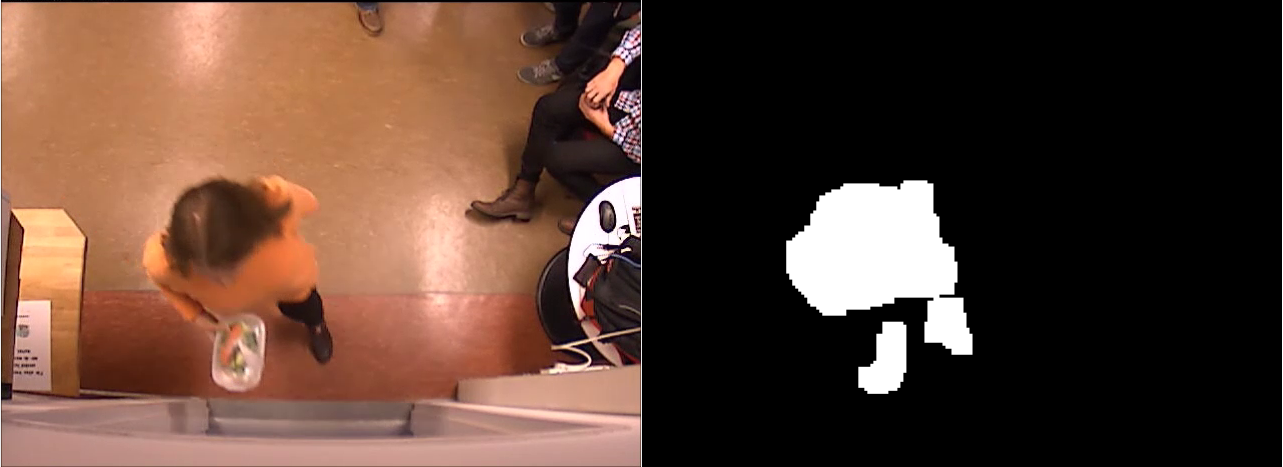
\includegraphics[width=\linewidth]{images/bg_success.png}
	\caption[An example of a successful detection using background subtraction.]{\textit{The left image shows a moving person who is detected by the background subtractor. The right image shows the binary image generated from the left image.
	}}
	\label{fig:bg_success}  %Skapar referens till figuren
\end{figure}

\begin{figure}[htb]
	\centering
	
\includegraphics[width=\linewidth]{images/bg_fail.png}
	\caption[An example of a failed detection detection using background subtraction.]{\textit{The left image shows a persons who is not detected by the background subtractor, because of insufficient movement. The right image shows the binary image generated from the left image. 
	}}
	\label{fig:bg_fail}  %Skapar referens till figuren
\end{figure}

